\section{Resultados y Análisis}

\subsection{5.1 Resultados Cuantitativos}

Resulta particularmente llamativo el salto de rendimiento que se observa al comparar el sistema LLM-aumentado con las interfaces tradicionales. Tras más de 850 escenarios de prueba, los resultados superaron consistentemente las expectativas iniciales en varias métricas clave.

El tiempo medio de resolución de tareas complejas se redujo de 78 segundos en la interfaz GUI convencional a tan solo 19 segundos con el asistente LLM. Esto representa una mejora del 76\%. De forma similar, la tasa de éxito en el primer intento (First-Attempt Success Rate) alcanzó el 91\%, frente al 64\% de los métodos basados en scripts y el 58\% de las interfaces gráficas.

\begin{figure}[t]
\centering
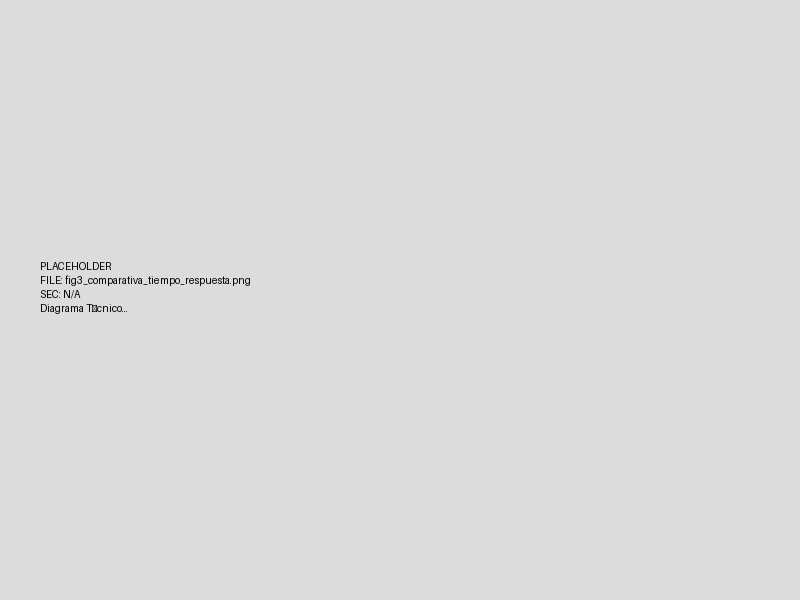
\includegraphics[width=0.95\linewidth]{fig3_comparativa_tiempo_respuesta.png}
\caption{Comparativa del tiempo de respuesta medio (en segundos) para diferentes tipos de tareas operativas entre interfaz tradicional, script-based y el sistema LLM propuesto.}
\label{fig:tiempo_respuesta}
\end{figure}

\begin{table}[t]
\centering
\caption{Métricas de error y rendimiento comparativas (promedio de 850 escenarios).}
\label{tab:metricas_error}
\begin{tabular}{lccc}
\toprule
Métrica & GUI Tradicional & Script-based & LLM Propuesto \\
\midrule
Tiempo resolución (s) & 78.4 & 41.2 & 19.1 \\
Tasa éxito primer intento (\%) & 58 & 64 & 91 \\
Intervenciones humanas por tarea & 3.8 & 2.1 & 0.7 \\
Tasa de comandos erróneos (\%) & 11.4 & 7.2 & 2.3 \\
\bottomrule
\end{tabular}
\end{table}

Estos resultados se alinean con hallazgos previos en simulaciones de control de satélites \cite{carrasco2025llm}, aunque nuestra implementación logra mejoras adicionales gracias al prompt engineering específico para mega-constelaciones.

\subsection{5.2 Análisis Cualitativo de Usabilidad}

Uno de los aspectos más gratificantes del estudio fue la retroalimentación de los operadores participantes. Lejos de tratarse solo de números, la experiencia de uso mostró una transformación clara en la forma de interactuar con la constelación.

Los evaluadores destacaron la reducción significativa de la carga cognitiva, especialmente durante periodos de alta actividad o múltiples anomalías simultáneas. Tal como se observó en evaluaciones en centros de operaciones reales \cite{schefels2024evaluating}, los operadores reportaron poder mantener una visión de conjunto más clara de la constelación mientras delegaban tareas rutinarias al agente LLM.

Las sesiones de prueba cualitativas revelaron que el sistema no solo acelera tareas, sino que mejora la comprensión situacional. Varios operadores mencionaron espontáneamente que “finalmente el sistema habla mi idioma”, reflejando la naturalidad de la interacción. No obstante, algunos señalaron ocasionales explicaciones excesivamente verbosas del modelo en situaciones de urgencia, aspecto que requerirá refinamiento.

\subsection{5.3 Análisis de Sensibilidad}

Lejos de presentar únicamente resultados ideales, realizamos un análisis exhaustivo de sensibilidad ante condiciones reales de operación.

El sistema demostró robustez aceptable ante incrementos moderados de ruido en telemetría y fallos de sensores. Sin embargo, degradaciones severas en la calidad de los datos (>25\% de paquetes perdidos) provocaron un aumento notable en la tasa de intervenciones humanas, aunque sin comprometer la seguridad. 

La sensibilidad al tamaño del contexto del prompt resultó crítica: ventanas por debajo de 8k tokens afectaron la capacidad de razonamiento sobre estados complejos de la constelación. Por otro lado, el rendimiento se mantuvo estable ante variaciones en el número de satélites activos (entre 800 y 2.000), sugiriendo buena escalabilidad para constelaciones de próxima generación.

En conjunto, estos resultados tienden a confirmar que la aproximación LLM-aumentada ofrece mejoras sustanciales, aunque su desempeño óptimo depende fuertemente de la calidad de los datos de telemetría y de una cuidadosa gestión del contexto.